\documentclass[11pt,oneside]{article}
\usepackage{geometry}                % See geometry.pdf to learn the layout options. There are lots.
\geometry{letterpaper}                   % ... or a4paper or a5paper or ... 
%\geometry{landscape}                % Activate for for rotated page geometry
\usepackage{fullpage}
\usepackage{graphicx}
\usepackage{amssymb}


%Special formatting packages
%\usepackage{datetime}
%\usepackage{fmtcount}
%\usepackage{timestamp}
\usepackage{fancyhdr}  %fancy headers/footers
\usepackage{pdfpages}  %input pdf pages
\usepackage{everypage} %allow repeating element on each page (for white-out of page numbers)
%\usepackage{tocloft} %table of contents customization
\usepackage{epstopdf}
\usepackage[pdftitle={Rejecta Mathematica Vol. 1, No. 1},pdfauthor={Rejecta Publications, Inc.},pdfsubject={Journal of Mathematical Science},pdfkeywords={journal, rejected paper, math, science, open access},bookmarks=true,colorlinks=true,linkcolor=black,urlcolor=black]{hyperref} %PDF bookmarks and links
%\usepackage{draftcopy} %for Proofs (dvips only)

\DeclareGraphicsRule{.tif}{png}{.png}{`convert #1 `dirname #1`/`basename #1 .tif`.png}

\if 0
%%%%%
% Draft Copy (PDF-latex)
%%%%%
\usepackage{type1cm}
\usepackage{eso-pic}
\usepackage{color}
\makeatletter
\AddToShipoutPicture{%
            \setlength{\@tempdimb}{.5\paperwidth}%
            \setlength{\@tempdimc}{.5\paperheight}%
            \setlength{\unitlength}{1pt}%
            \put(\strip@pt\@tempdimb,\strip@pt\@tempdimc){%
        \makebox(0,0){\rotatebox{45}{\textcolor[gray]{0.75}%
        {\fontsize{6cm}{6cm}\selectfont{DRAFT}}}}%
            }%
}
\makeatother
%%%%%%
% End Draft Copy
%%%%%%
\fi

\pagestyle{fancy}

%Redefine TOC contents title


\begin{document}


%%%%%%%%%%%%%%%%%%%%%%%%%%%%%%%%%%%%%%%%%%%%%%
%Cover Page

%TOC Name
%\renewcommand{\contentsname}{\textsf{Contents}} %new contents title font
\renewcommand{\contentsname}{} %empty contents title

\phantomsection
\addtocontents{toc}{\protect\setcounter{tocdepth}{0}}
\addcontentsline{toc}{section}{\textsf{Rejecta Mathematica Vol. 1, No. 1}}
\addtocontents{toc}{\protect\setcounter{tocdepth}{2}}


%\textheight = 639pt %extend hight of text for this page
%\footskip = 60pt %move down footer for some extra space
\fancyhead{} 
\renewcommand{\headrulewidth}{0.0pt} 
\fancyfoot{} 
%\fancyfoot[C]{2009 Rejecta Publications, Inc.}
\fancyfoot[L]{
\vspace{-1.45cm}
\begin{center}
\footnotesize{2009 Rejecta Publications, Inc.}
\end{center}
\footnotesize{\textsf{This work is published under the Creative Commons Attribution-NonCommercial License.\\
~~~~~~~~~\textbf{License}  \href{http://creativecommons.org/licenses/by-nc/2.5/legalcode}{http://creativecommons.org/licenses/by-nc/2.5/legalcode}\\
~~~~~~~~~\textbf{Human-Readable Summary}  \href{http://creativecommons.org/licenses/by-nc/2.5/}{http://creativecommons.org/licenses/by-nc/2.5/} }}
}
\begin{picture}(0,0)(16,664)  %(width, height)(-x,y) in mm
		\put(0,0){
\includegraphics[width=.048\linewidth]{cc}}
\end{picture}

\begin{center}
 \href{http://math.rejecta.org}{
\includegraphics[width=\linewidth]{logo}}
\end{center}
%\vspace{-.5in}
\vspace{-.53in}
\begin{flushright}
Volume 1, Number 1~|~July 2009\\
{\footnotesize ISSN 1948-8351}\\
\href{http://math.rejecta.org}{\textsf{math.rejecta.org}}\\
\end{flushright}


\hfill
%\vspace{.1in}

\noindent\small{\emph{Rejecta Mathematica is an open access, online journal that publishes papers that have been rejected from peer-reviewed journals in the mathematical sciences. Each paper is accompanied by an open letter from its authors discussing the original review process and stating the case for its value to the research community.}}

\hfill
%\vspace{.01in}

\vspace{-1cm}
\begin{center}
\tableofcontents
\end{center}

\noindent \hrulefill
%\hfill


%\hfill
%\hfill
%\hfill

\begin{flushright}
%Editors\\
\emph{Michael  Wakin --- Christopher  Rozell --- Mark  Davenport --- Jason  Laska}\\
%\end{flushright}
%
%
%\begin{flushright}
\href{mailto:editors@rejecta.org}{{\footnotesize \textsf{editors@rejecta.org}}}\\
\end{flushright}


%End Cover Page
\newpage








%%%%%%%%%%%%%%%%%%%%%%%%%%%%%%%%%%%%%%%%%%%%%%
%Content

%\textheight = 609pt %undo changed text height
%\footskip = 30pt %undo footer space

%Declare footer for whole document
\fancyfoot{} % clear all footer fields 
\fancyfoot[R]{\thepage}
%Fine-grained control over picture
\AddEverypageHook{
	\begin{picture}(0,0)(-32,684)  %(width, height)(-x,y) in mm (-60,674) for ``right footer''
						       % (-32,684) when no timestamp
		\put(0,0){
\includegraphics[width=.02\linewidth]{cc}}
	\end{picture}
}
\fancyfoot[L]{\href{http://math.rejecta.org}{\emph{\small{Rejecta Mathematica}}}} 
\fancyfoot[C]{\small{Vol. 1, No. 1, July 2009}\\\hfill\\\hfill\\\tiny{\textsf{~~~~~This work is published under the Creative Commons Attribution-NonCommercial License. \href{http://creativecommons.org/licenses/by-nc/2.5/legalcode}{http://creativecommons.org/licenses/by-nc/2.5/legalcode}}}}
\renewcommand{\footrulewidth}{0.4pt} 

%Start page numbering
\setcounter{page}{1}


%Letter from the editors...
\phantomsection
\addcontentsline{toc}{section}{\small{\textsf{Letter from the Editors}}}
\fancyhead{} 
\fancyhead[L]{
	\includegraphics[width=.08\linewidth]{logoNotext}\vspace{.2cm}\\
	\large{\textit{\textsf{LETTER FROM THE EDITORS}}}
} 
\fancyhead[R]{{\scriptsize{\textbf{
	%Letter from the editors\\
	\emph{Rejecta Mathematica}, Vol. 1, No. 1, pp. 1-3, July 2009\\
	2009 Rejecta Publications\\
	\vspace{-.15cm}
	\href{http://math.rejecta.org}{math.rejecta.org}%
}}}}
\renewcommand{\headrulewidth}{0.4pt} 
\includepdf[pages=-,pagecommand={\pagestyle{fancy}},noautoscale, scale=.9,offset={0pt -40pt}]{author_source/coverletter/coverletter25june2009} 



%For different bookmark and TOC names
%\texorpdfstring{TEXstring}{PDFstring}


%This just adds text without a bookmark or section, etc.
\addtocontents{toc}{
	\hrulefill~\textsf{Articles}~\hrulefill\\
}





%Joshi and Boyd
\phantomsection
\addcontentsline{toc}{section}{\small{\textsf{Subspaces that Minimize the Condition Number of a Matrix}}}
\addtocontents{toc}{
	\hbox{\textit{\footnotesize{\textsf{Siddharth Joshi and Stephen Boyd}}}}
}
%\phantomsection
%\addcontentsline{toc}{subsection}{\textsf{\small{Open Letter}}}
\fancyhead{} 
\fancyhead[L]{
	\includegraphics[width=.08\linewidth]{logoNotext}\vspace{.2cm}\\
	\large{\textit{\textsf{ARTICLE}}}
} 
\fancyhead[R]{{\scriptsize{\textbf{
	Siddharth Joshi and Stephen Boyd\\
	Subspaces that Minimize the Condition Number of a Matrix\\
	\textit{Rejecta Mathematica}, Vol. 1, No. 1, pp. 4-9, July 2009\\
	2009 Rejecta Publications\\
	\vspace{-.15cm}
	\href{http://math.rejecta.org}{math.rejecta.org}%
}}}}
\renewcommand{\headrulewidth}{0.4pt} 
\includepdf[pages=-,pagecommand={\pagestyle{fancy}},noautoscale, scale=.9,offset={0pt -40pt}]{author_source/JoshiBoyd/openletter/openletter} 
%\phantomsection
%\addcontentsline{toc}{subsection}{\textsf{\small{Paper}}}
\fancyhead{} 
\fancyhead[L]{\small{{S. Joshi and S. Boyd}}}
\fancyhead[R]{\small{\textit{\textsf{Subspaces that Minimize the Condition Number of a Matrix}}}} 
\renewcommand{\headrulewidth}{0.4pt} 
\includepdf[pages=-,pagecommand={\pagestyle{fancy}},noautoscale, scale=.9]{author_source/JoshiBoyd/article/min_cond_sub} 


%Doron Zeilberger
\phantomsection
\addcontentsline{toc}{section}{\small{\textsf{Automatic CounTilings}}}
\addtocontents{toc}{
	\hbox{\textit{\footnotesize{\textsf{Doron Zeilberger}}}}
}
%\phantomsection
%\addcontentsline{toc}{subsection}{\textsf{\small{Open Letter}}}
\fancyhead{} 
\fancyhead[L]{
	\includegraphics[width=.08\linewidth]{logoNotext}\vspace{.2cm}\\
	\large{\textit{\textsf{ARTICLE}}}
} 
\fancyhead[R]{{\scriptsize{\textbf{
	Doron Zeilberger\\
	Automatic CounTilings\\
	\emph{Rejecta Mathematica}, Vol. 1, No. 1, pp. 10-17, July 2009\\
	2009 Rejecta Publications\\
	\vspace{-.15cm}
	\href{http://math.rejecta.org}{math.rejecta.org}%
}}}}
\renewcommand{\headrulewidth}{0.4pt} 
\includepdf[pages=-,pagecommand={\pagestyle{fancy}},noautoscale, scale=.9,offset={0pt -80pt}]{author_source/DoronZeilberger/openletter/openletter} 
%\phantomsection
%\addcontentsline{toc}{subsection}{\textsf{\small{Paper}}}
\fancyhead{} 
\fancyhead[L]{\small{{D. Zeilberger}}}
\fancyhead[R]{\small{\textit{\textsf{Automatic CounTilings}}}} 
\renewcommand{\headrulewidth}{0.4pt} 
%White out page numbers
%-- note: once everypage is used, it cannot be undone,
%-- 	        thus, conditionals must be used
%-- Define variable: epageDZ
\newif\ifepageDZ
\epageDZtrue
\AddEverypageHook{
\ifepageDZ
	 \begin{picture}(0,0)(0,635)  %(width, height)(x,y) in mm %(0,600) for scale=.8 %(0,635) for scale=.9
		\put(0,0){\colorbox{white}{
				\parbox{\columnwidth}{\hfill\\\hfill}\\
			}}
	\end{picture}
\else
\fi
}
\includepdf[pages=-,pagecommand={\pagestyle{fancy}},noautoscale, scale=.9,offset={20pt -30pt}]{author_source/DoronZeilberger/article/tilings} 
\epageDZfalse




%Ezra Miller
\phantomsection
\addcontentsline{toc}{section}{\small{\textsf{Alexander Duality for Monomial Ideals and their Resolutions}}}
\addtocontents{toc}{
	\hbox{\textit{\footnotesize{\textsf{Ezra Miller}}}}
}
%\phantomsection
%\addcontentsline{toc}{subsection}{\textsf{\small{Open Letter}}}
\fancyhead{} 
\fancyhead[L]{
	\includegraphics[width=.08\linewidth]{logoNotext}\vspace{.2cm}\\
	\large{\textit{\textsf{ARTICLE}}}
} 
\fancyhead[R]{{\scriptsize{\textbf{
	Ezra Miller\\
	Alexander Duality for Monomial Ideals and their Resolutions\\
	\emph{Rejecta Mathematica}, Vol. 1, No. 1, pp. 18-57, July 2009\\
	2009 Rejecta Publications\\
	\vspace{-.15cm}
	\href{http://math.rejecta.org}{math.rejecta.org}%
}}}}
\renewcommand{\headrulewidth}{0.4pt} 
\includepdf[pages=-,pagecommand={\pagestyle{fancy}},noautoscale, scale=.9,offset={0pt -20pt}]{author_source/EzraMiller/openletter/openletter} 
%\phantomsection
%\addcontentsline{toc}{subsection}{\textsf{\small{Paper}}}
\fancyhead{} 
\fancyhead[L]{\small{{E. Miller}}}
\fancyhead[R]{\small{\textit{\textsf{Alexander Duality for Monomial Ideals and their Resolutions}}}} 
\renewcommand{\headrulewidth}{0.4pt} 
\includepdf[pages=-,pagecommand={\pagestyle{fancy}},noautoscale, scale=.9]{author_source/EzraMiller/article/alexdual080225} 
 
 
%Gary Harper
\phantomsection
\addcontentsline{toc}{section}{\small{\textsf{Meaning-Imposers versus Meaning-Derivers}}}
\addtocontents{toc}{
	\hbox{\textit{\footnotesize{\textsf{Gary Harper}}}}
}
%\phantomsection
%\addcontentsline{toc}{subsection}{\textsf{\small{Open Letter}}}
\fancyhead{} 
\fancyhead[L]{
	\includegraphics[width=.08\linewidth]{logoNotext}\vspace{.2cm}\\
	\large{\textit{\textsf{ARTICLE}}}
} 
\fancyhead[R]{{\scriptsize{\textbf{
	Gary Harper\\
	Meaning-Imposers versus Meaning-Derivers\\
	\emph{Rejecta Mathematica}, Vol. 1, No. 1, pp. 58-83, July 2009\\
	2009 Rejecta Publications\\
	\vspace{-.15cm}
	\href{http://math.rejecta.org}{math.rejecta.org}%
}}}}
\renewcommand{\headrulewidth}{0.4pt} 
\includepdf[pages=-,pagecommand={\pagestyle{fancy}},noautoscale, scale=.85,offset={0pt -30pt}]{author_source/GaryHarper/openletter/openletter} 
%\phantomsection
%\addcontentsline{toc}{subsection}{\textsf{\small{Paper}}}
\fancyhead{} 
\fancyhead[L]{\small{{G. Harper}}}
\fancyhead[R]{\small{\textit{\textsf{Meaning-Imposers versus Meaning-Derivers}}}} 
\renewcommand{\headrulewidth}{0.4pt} 
\includepdf[pages=-,pagecommand={\pagestyle{fancy}},noautoscale, scale=.85]{author_source/GaryHarper/article/article} 




%Neelsh, Baraniuk
\phantomsection
\addcontentsline{toc}{section}{\small{\textsf{WInHD: Wavelet-based Inverse Halftoning via Deconvolution}}}
\addtocontents{toc}{
	\hbox{\textit{\footnotesize{\textsf{Ramesh Neelamani and Richard Baraniuk}}}}
}
%\phantomsection
%\addcontentsline{toc}{subsection}{\textsf{\small{Open Letter}}}
\fancyhead{} 
\fancyhead[L]{
	\includegraphics[width=.08\linewidth]{logoNotext}\vspace{.2cm}\\
	\large{\textit{\textsf{ARTICLE}}}
} 
\fancyhead[R]{{\scriptsize{\textbf{
	Ramesh Neelamani and Richard Baraniuk\\
	WInHD: Wavelet-based Inverse Halftoning via Deconvolution\\
	\emph{Rejecta Mathematica}, Vol. 1, No. 1, pp. 84-103, July 2009\\
	2009 Rejecta Publications\\
	\vspace{-.15cm}
	\href{http://math.rejecta.org}{math.rejecta.org}%
}}}}
\renewcommand{\headrulewidth}{0.4pt} 
\includepdf[pages=-,pagecommand={\pagestyle{fancy}},noautoscale, scale=.88,offset={0pt -40pt}]{author_source/NeelshBaraniuk/openletter/openletter} 
%\phantomsection
%\addcontentsline{toc}{subsection}{\textsf{\small{Paper}}}
\fancyhead{} 
\fancyhead[L]{\small{{R. Neelamani and R. Baraniuk}}}
\fancyhead[R]{\small{\textit{\textsf{WInHD: Wavelet-based Inverse Halftoning via Deconvolution}}}} 
\renewcommand{\headrulewidth}{0.4pt} 
\includepdf[pages=-,pagecommand={\pagestyle{fancy}},noautoscale, scale=.9,offset={0pt -10pt}]{author_source/NeelshBaraniuk/article/article} 
\newpage



%Marni Sheppeard
\phantomsection
\addcontentsline{toc}{section}{\small{\textsf{Mass Matrix Transforms in Qubit Field Theory}}}
\addtocontents{toc}{
	\hbox{\textit{\footnotesize{\textsf{Marni Sheppeard}}}}
}
%\phantomsection
%\addcontentsline{toc}{subsection}{\textsf{\small{Open Letter}}}
\fancyhead{} 
\fancyhead[L]{
	\includegraphics[width=.08\linewidth]{logoNotext}\vspace{.2cm}\\
	\large{\textit{\textsf{ARTICLE}}}
} 
\fancyhead[R]{{\scriptsize{\textbf{
	Marni Sheppeard\\
	Mass Matrix Transforms in Qubit Field Theory\\
	\emph{Rejecta Mathematica}, Vol. 1, No. 1, pp. 104-109, July 2009\\
	2009 Rejecta Publications\\
	\vspace{-.15cm}
	\href{http://math.rejecta.org}{math.rejecta.org}%
}}}}
\renewcommand{\headrulewidth}{0.4pt} 
\includepdf[pages=-,pagecommand={\pagestyle{fancy}},noautoscale, scale=.9,offset={0pt -60pt}]{author_source/MarniSheppeard/openletter/openletter} 
%\phantomsection
%\addcontentsline{toc}{subsection}{\textsf{\small{Paper}}}
\fancyhead{} 
\fancyhead[L]{\small{{M. Sheppeard}}}
\fancyhead[R]{\small{\textit{\textsf{Mass Matrix Transforms in Qubit Field Theory}}}} 
\renewcommand{\headrulewidth}{0.4pt} 
\includepdf[pages=-,pagecommand={\pagestyle{fancy}},noautoscale, scale=.85]{author_source/MarniSheppeard/article/fouriermass07} 





\end{document}  